SocratiCode dispone de pantallas dedicadas al acceso y la gestión de la cuenta de usuario. Todas ellas mantienen el mismo estilo visual oscuro que el entorno de trabajo principal. La \autoref{fig:auth-pantallas} muestra las tres vistas principales: el inicio de sesión, el registro de una cuenta nueva y la pantalla de perfil, donde el alumno puede consultar y editar sus datos personales.

\begin{figure}[Pantallas de usuario]{fig:auth-pantallas}{Pantallas de inicio de sesión, registro y perfil de usuario de SocratiCode.}
    \centering
    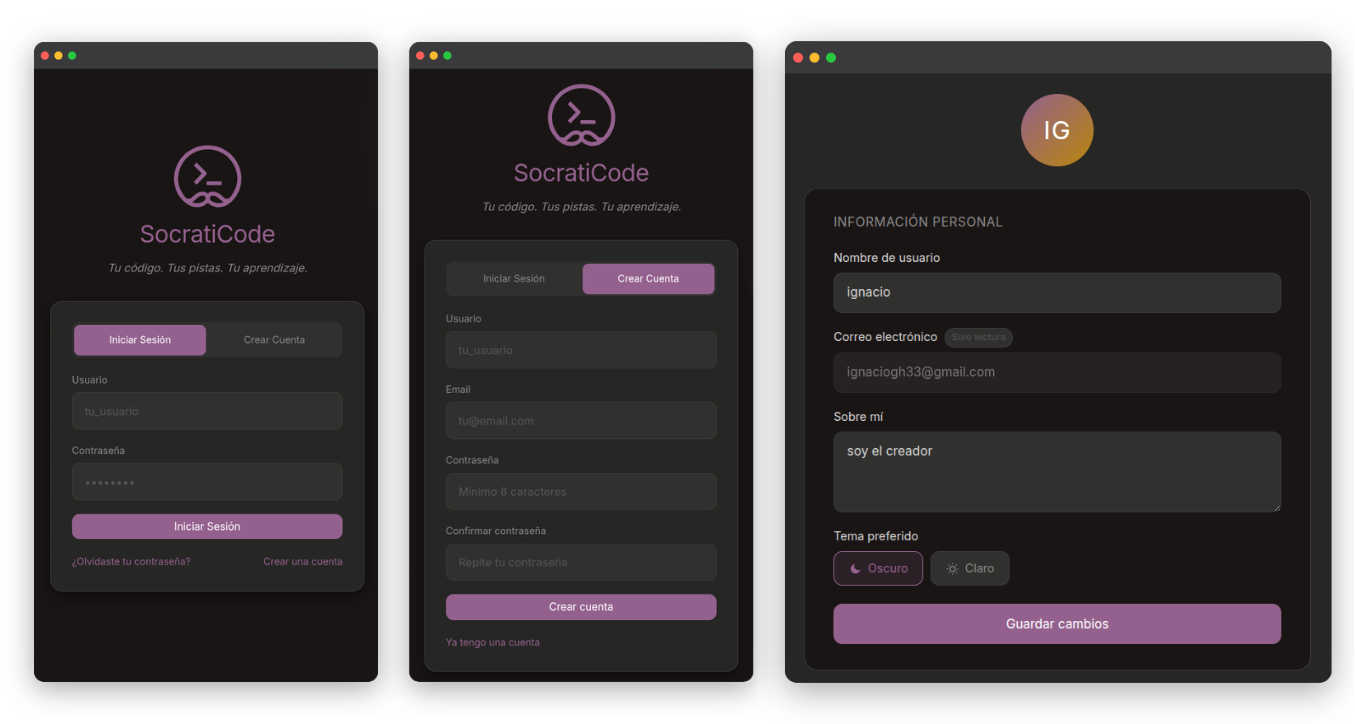
\includegraphics[width=\textwidth]{./pantallas/pantallas_usuario.png}
\end{figure}

Las pantallas de cambio de contraseña y del flujo completo de recuperación de acceso por correo electrónico se recogen en el \autoref{CAP:AP_INTERFACES}.
